\section{Public key cryptography}

Public key cryptography is the backbone of most distributed systems. It provides both a way to encrypt a message and to confirm the source of a message, without the need to agree upon a shared key. The most common implementation of this idea is the RSA encryption algorithm, named after inventors Rivest, Shamir and Adleman \cite{rsa-patent}. 

\subsection{Basics}

If two parties wanted to safely exchanges messages before public key cryptography was invented, they had to agree on a common code. This code is referred to as a cipher. An example of such an encryption system is the Ceasar cipher \cite{ceasar-cypher}. With a Ceasar cipher, every character of the message is offset by an agreed upon number. Yet, if a third party manages to intercept the transmission of the cipher itself, all encrypted messages can be decoded. Thus, a trusted third party network is required to safely exchange the cipher.

Public key cryptography uses a pair of hashes instead. These hashes are referred to as the keys. The keys are algorithmically generated so that they are cryptographically connected. This means that a message encrypted with one key can only be decrypted with the other key and vice versa \cite{rsa-paper-explanation}.

One of these keys can be broadcasted. As a result, everyone knows that this key is connected to the owner's identity. Therefore, it is referred to as the public key. The other key will be held privately. It is very important that nobody except the owner knows the content of this key, as it is used to prove the owner's identity. It is therefore referred to as the private key.

Because no cipher has to be exchanged, a trusted exchange middleman is no longer necessary. This eliminates a key weakness of cipher encryption.

\subsection{Uses: encryption and source validation}

A first use case of public key cryptography is encryption. If Alice wants to send a message to Bob, she encrypts her message with Bob's public key. As a result, only Bob can decrypt this message as only Bob knows the corresponding private key. The message can now be sent over any insecure network, such as the internet, email or even carrier pigeon, without any danger of leaking its contents.

Besides encryption, public key cryptography can also be used for source validation. If Alice wants to broadcast a message to the world, she can encrypt the message with her private key. As the encrypted message can only be decrypted with Alice's public key, everyone knows that only Alice could have encrypted it. This case is referred to as a digital signature, as Alice signed the message with her private key. 

For full security, a secure message is often first encrypted with the private key of the sender and then with the public key of the recipient. Now only the recipient can decrypt the message and can then confirm the origin of the message. This full process is modeled in figure \ref{fig:rsa-diagram}.

\begin{figure}[h]
\centering
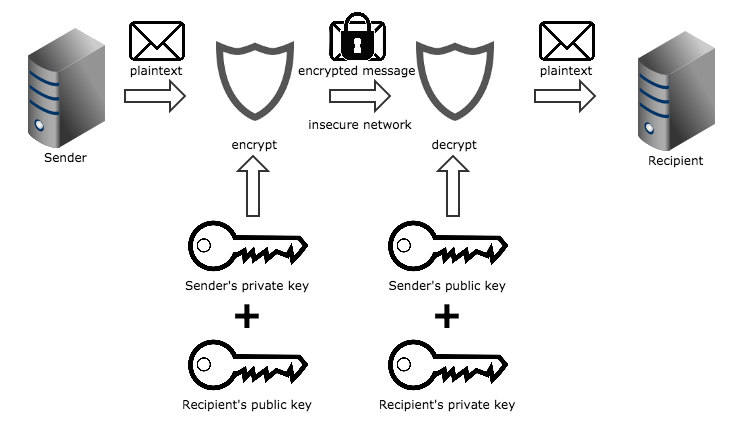
\includegraphics[width=0.8\textwidth]{paper-images/rsa-diagram.png}
\caption{}
\label{fig:rsa-diagram}
\end{figure}

